\documentclass[9pt]{beamer}
\usepackage[sfdefault]{roboto}
\usepackage{styles/fluxmacros}
\usefolder{styles}
\usetheme[style=asphalt]{flux}
\usepackage{xcolor}
\usepackage{color}
\usepackage{amsmath}
\usepackage{amssymb}
\usepackage{graphicx}
\usepackage{latexsym}
\usepackage[T1]{fontenc}
\usepackage[utf8]{inputenc}
\usepackage{wrapfig}
\usepackage{siunitx}
%\usepackage{times}
\usepackage{tikz}
\usepackage{verbatim}
\usepackage{multimedia}
\usepackage{hyperref}
\usepackage{thumbpdf}
\usepackage{%
    pgf,%
    pgfarrows,%
    pgfnodes,%
    pgfautomata,%
    pgfheaps,%
    pgfshade%
}
\usepackage{url}
\usepackage{empheq}
\usepackage{fancybox}
\usepackage{esint}
\usepackage{lipsum}
\usepackage{listings}
\usepackage{mathptmx}
\usepackage{helvet}
\usepackage{tikz}%
\usepackage{circuitikz}
\usepackage{csvsimple}
\usepackage{pgfplots}
\usepackage{multimedia}
\usepackage{proba}
\usepackage[absolute,overlay]{textpos}
\usepackage{bibunits}
\usepackage{tcolorbox}
\usepackage{qrcode}
%\usepackage[texcoord,%
%            grid,%
%            gridunit=mm,%
%            gridcolor=red!60,%
%           subgridcolor=black!60%
%            ]{eso-pic}
\usepackage{enumerate}
\usepackage[makeroom]{cancel}
\usepackage{epstopdf}
\usepackage{booktabs}
\usepackage{calc}
\usepackage{enumitem}
\usepackage{algorithm}
\usepackage{algpseudocode}
\usepackage{pifont}
\setbeamercovered{transparent}
% Informations

\epstopdfsetup{outdir=./}
\mode<presentation>
{
    \useinnertheme{progressbar}
}
%\setbeamertemplate{items}[ball]
%~~~~~~~~~~~~~~~~~~~~~~~~~~~~~~~~~~~~~~~~~~~~-~~~~~~~~~~~~~~~~~~~~~~~~~~~~~~~~~~
%~~~~~~~~~~~~~~~~~~~~~~~~~~~~~~~~~~~~~~~~~~~~~-~~~~~~~~~~~~~~~~~~~~~~~~~~~~~~~~~
% Informations
\defaultbibliography{main}
%
\title{\Huge{Estimaci\'{o}n m\'{a}ximo veros\'{i}mil }\\
    \Huge{
        \textbf{
        para un sistema SEIR estoc\'{a}stico
        }
    }
}
\subtitle{%
        \textbf{
            \textcolor{gray}{
                 con una aplicaci\'{o}n COVID-19%
            }
       }
    \\
    \normalsize{October 25, 2023, 56 Congreso SMM }
    } 
    
%
\author{
    \normalsize{%
        CONAHCYT-UNISON-UNAM: FDV, FBL, SDIV
    }
}
%
\titlegraphic{assets/logoUNISON-UNAM-CONACHYT.png}
%~~~~~~~~~~~~~~~~~~~~~~~~~~~~~~~~~~~~~~~~~~~~~~~~~~~~~~~~~~~~~~~~~~~~~~~~~~~~~~
%%%%%%%%%%%%%%%%%%%%%%%%%%%%%%%%%%%%%%%%%%%%%%%%%%%%%%%%%%%%%%%%%%%%%%%%%%%%%%%%
\def\Q#1#2{\frac{\partial #1}{\partial #2}}
\usetikzlibrary{arrows,shapes}
\pgfplotsset{compat=1.14}
% \pgfplotstableread[col sep = comma]{noise/Images/Introduction/gbm.csv}\mydata
\epstopdfsetup{outdir=./}
%%%%%%%%%%%%%%%%%%%%%%%%%%%%%%%%%%%%%%%%%%%%%%%%%%%%%%%%%%%%%%%%%%%%%%%%%%%%%%%%
%-----------------------------ExtrasDeTercerPresentacion
%--------------------------------Fancyboxes-------------------------------------
\definecolor{myblue}{rgb}{.8, .8, 1}
\definecolor{azure(colorwheel)}{rgb}{0.0, 0.5, 1.0}
\definecolor{shadecolor}{cmyk}{0,0,0.41,0}
\newcommand*\mybluebox[1]{%
    \colorbox{myblue}{\hspace{1em}#1\hspace{1em}}
}
\newcommand*\myyellowbox[1]{%
    \colorbox{darkyellow}{\hspace{1em}#1\hspace{1em}}
}
%--------------------------------------------------------------------------
\definecolor{shadecolor}{cmyk}{0,0,0.41,0}
\definecolor{light-blue}{cmyk}{0.25,0,0,0}
\newsavebox{\mysaveboxM} % M for math
\newsavebox{\mysaveboxT} % T for text
\newcommand*\Garybox[2][Example]{%
    \sbox{\mysaveboxM}{#2}%
        \sbox{\mysaveboxT}{\fcolorbox{black}{light-blue}{#1}}%
            \sbox{\mysaveboxM}{%
    \parbox[b][\ht\mysaveboxM+.5\ht\mysaveboxT+.5\dp\mysaveboxT][b]{%
        \wd\mysaveboxM}{#2}%
    }%
    \sbox{\mysaveboxM}{%
        \fcolorbox{black}{shadecolor}{%
        \makebox[\linewidth-10em]{\usebox{\mysaveboxM}}%
        }%
    }%
    \usebox{\mysaveboxM}%
    \makebox[0pt][r]{%
        \makebox[\wd\mysaveboxM][c]{%
            \raisebox{\ht\mysaveboxM-0.5\ht\mysaveboxT
            +0.5\dp\mysaveboxT-0.5\fboxrule}{\usebox{\mysaveboxT}}%
        }%
    }%
}
\newcommand\Fontvi{\fontsize{7}{7.2}\selectfont}
%%%%%%%%%%%%%%%%%%%%%%%%%%%%%%%%%%%%%%%%%%%%
\definecolor{kugreen}{RGB}{50,93,61}
\definecolor{kugreenlys}{RGB}{132,158,139}
\definecolor{kugreenlyslys}{RGB}{173,190,177}
\definecolor{kugreenlyslyslys}{RGB}{214,223,216}
\definecolor{greenArea}{RGB}{124,252,124}
\definecolor{hellmagenta}{rgb}{1,0.75,0.9}
\definecolor{hellcyan}{rgb}{0.75,1,0.9}
\definecolor{hellgelb}{rgb}{1,1,0.8}
\definecolor{colKeys}{rgb}{0,0,1}
\definecolor{colIdentifier}{rgb}{0,0,0}
\definecolor{colComments}{rgb}{1,0,0}
\definecolor{colString}{rgb}{0,0.5,0}
\definecolor{darkyellow}{rgb}{1,0.9,0}
\setbeamercovered{transparent}
\lstset{%
    language=[AlLaTeX]TEX,%
    float=hbp,%
    basicstyle=\ttfamily\small, %\usepackage{cir}
    identifierstyle=\color{colIdentifier}, %
    keywordstyle=\color{colKeys}, %
    stringstyle=\color{colString}, %
    commentstyle=\color{colComments}, %
    columns=flexible, %
    tabsize=3, %
    frame=single, %
    extendedchars=true, %
    showspaces=false, %
    showstringspaces=false, %
    numbers=left, %
    numberstyle=\tiny, %
    breaklines=true, %
    backgroundcolor=\color{hellgelb}, %
    breakautoindent=true, %
    captionpos=b,%
    xleftmargin=18pt,%
    xrightmargin=\fboxsep%
}
\pgfplotsset{
    left segments/.code={\pgfmathsetmacro\leftsegments{#1}},
    left segments=3,
    left/.style args={#1:#2}{
        ybar interval,
        domain=#1:#2,
        samples=\leftsegments+1,
        x filter/.code=\pgfmathparse{\pgfmathresult}
       }
}
\DeclareMathOperator{\sign}{sgn}
\newcommand{\innerprod}[2]{\left\langle#1, #2\right\rangle}
\newcommand\bound{10} % bound number of points on each side of N
\newcommand\labelnum[3][]{
    \begin{scope}[font=\footnotesize,x=.3cm,#1]
      \foreach \mypt in {0,#2,...,\bound}{
        \draw(\mypt,0)circle[radius=2pt];
        \draw(-\mypt,0)circle[radius=2pt];
      }
      \draw(-\bound-5,0)--(\bound+5,0) node[pos=0, left]{$t$};
      \node(start)[at={(-\bound-4,0)},label=below:{$t_0=0$}]{$[$};
      \node(end)[at={(\bound+4,0)},label=below:{$T=Nh$}]{$]$};
      \node[%
          at={($(start)!.319!(end)$)},
          label=below:{
               $\underbrace{}_{h}$
            }%
            ]{\vphantom{$[$}};
      \node[at={($(start)!.57!(end)$)},label=below:{$t_{n+1}$}]{\vphantom{$[$}};
      \filldraw(0,0)circle[radius=2pt];
      \node[at={(-\bound-2,0)},above]{$\cdots$};
      \node[at={(\bound+2,0)},above]{$\cdots$};
      \node[at={(0,0)},above=5pt]{#3};
    \end{scope}
}
\usepackage{remreset}
\makeatletter
\@removefromreset{subsection}{section}
\makeatother
\definecolor{greenstrong}{rgb}{0.58,0.77,0.29}
\definecolor{redstrong}{rgb}{0.81,0.22,0.23}
\definecolor{fglisting}{gray}{0.3}
\definecolor{bglisting}{gray}{1}
\definecolor{fgshell}{gray}{1}
\definecolor{bgshell}{gray}{0.1}
\definecolor{bgshelllight}{gray}{0.8}
\definecolor{cadmiumorange}{rgb}{0.93, 0.53, 0.18}
\definecolor{capri}{rgb}{0.0, 0.75, 1.0}
%
\setcounter{subsection}{1}
\newcommand{\hl}[1]{\textbf{\textcolor{greenstrong}{#1}}}
\newcommand{\hb}[1]{\textbf{\textcolor{azure(colorwheel)}{#1}}}
\newcommand{\hlErr}[1]{\textcolor{redstrong}{\texttt{#1}}}
\newcommand{\hlOk}[1]{\textcolor{green}{\texttt{#1}}}
\newcommand{\hlInv}[1]{\colorbox{bgshell}{\textcolor{fgshell}{\texttt{#1}}}}
\newcommand{\unhl}[1]{\textcolor{gray}{#1}}
\newcommand{\clda}[0]{$\textcolor{blue}{\lambda}$}
\newcommand{\carr}[0]{$\textcolor{purple}{\rightarrow}$}
\newcommand{\cbind}[0]{\textbf{\texttt{$>\!\!>\!\!=$}}}
\newcommand{\codedots}[0]{\textcolor{mid-gray}{...}}

%
\tcbuselibrary{skins, breakable}
 \newtcolorbox{greenbox}[1]{%
        colback = green!5!white,
        colframe = green!55!black,
        fonttitle = \bfseries,
        title = #1 %
    }
\newtcolorbox{bluebox}[1]{%
        colback = blue!5!white,
        colframe = blue!55!black,
        fonttitle = \bfseries,
        title = #1
    }
%
\newtcolorbox{graybox}[1]{%
        colback = gray!5!white,
        colframe = gray!55!black,
        fonttitle = \bfseries,
        title = #1
    }
%
\newtcolorbox{yellowbox}[1]{%
        colback = yellow!5!white,
        colframe = yellow!55!black,
        fonttitle = \bfseries,
        title = #1
    }

\newcolumntype{P}[1]{>{\centering\arraybackslash}p{#1}}
\begin{document}
    \titlepage  
        \section{Motivation: MCMC Overfitting example}
            \subsection{Deterministic Formulation}
            \begin{frame}{CDMX Covid-19 data}
	%
	\begin{textblock*}{120mm}(3mm, 20mm)
		\only<1->{
			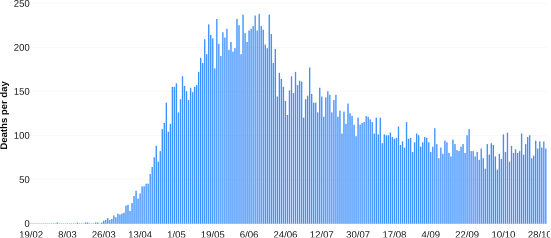
\includegraphics[width=\textwidth, keepaspectratio]{%
						assets/cdmx_dta.png
			}
		}	
	\end{textblock*}	
	%
	\begin{textblock*}{120mm}(70mm, 20mm)
		\only<2>{
			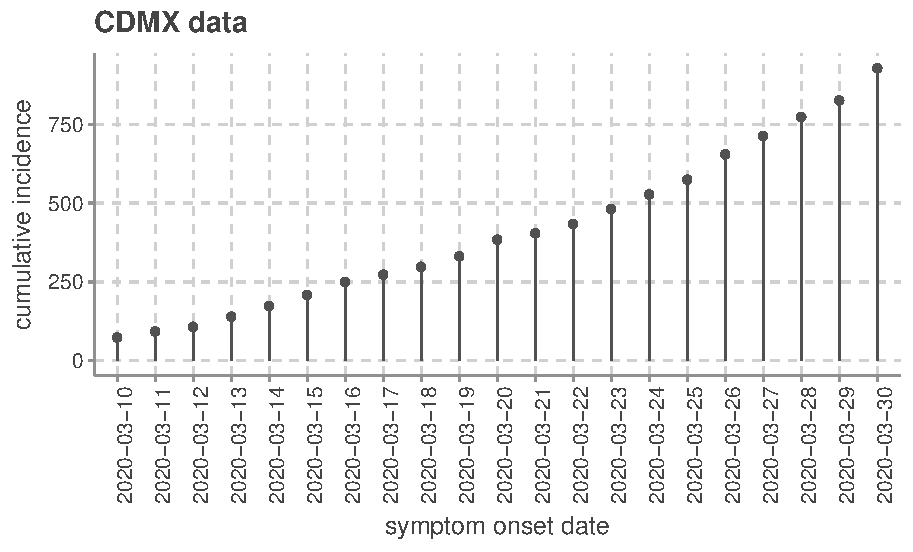
\includegraphics[width=0.4\textwidth, keepaspectratio]{%
				assets/cdmx_input_data}
		}
	\end{textblock*}
\end{frame}
%------------------------------------------------------------


\begin{frame}{First attempt: MCMC with a deterministic SEIRS structure}

	\begin{textblock*}{120mm}(0mm, 10mm)
		\only<1->{        
			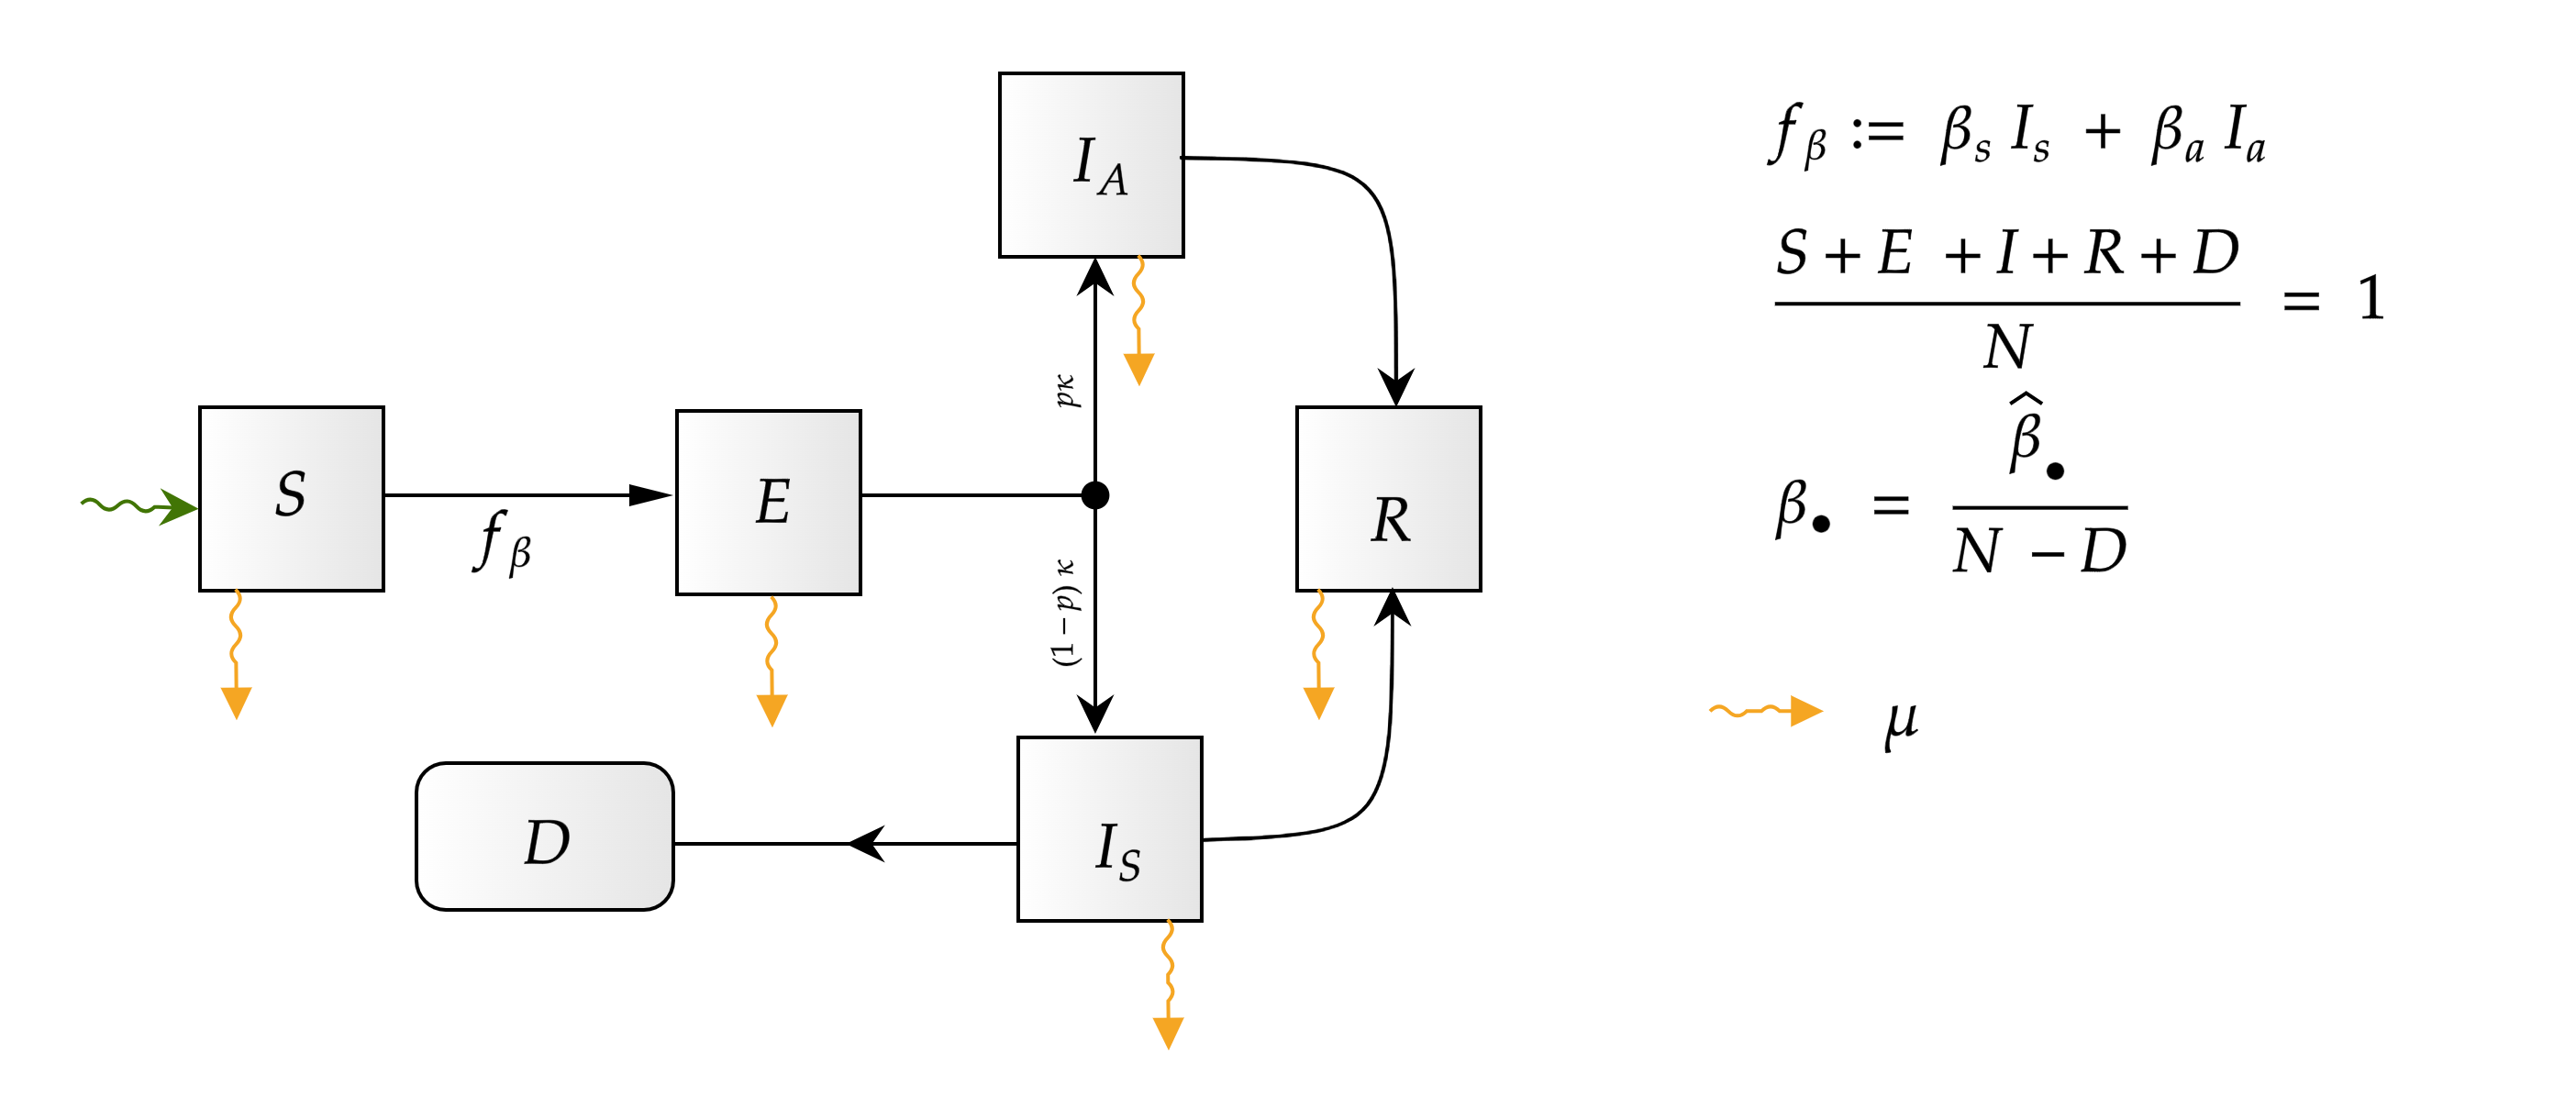
\includegraphics[width=\textwidth]{assets/stoSEIR_diagram.png} 
		}
	\end{textblock*}    
%    
%%    
	\begin{textblock*}{60mm}(0mm, 50mm)
		\only<2->{
			\begin{equation*}
				\label{eqn:base_dynamics}
				\begin{aligned}
					S'  &=
						\mu +\gamma R
						- \left(\mu  + f_{\beta} \right)  S
					\\
					E' & =  f_{\beta}S
						- (\kappa E + \mu E)
					\\
					{I_a}' &=
						p \kappa E
						- \big(\alpha_a + \mu \big)I_a
					\\
					{I_s}' &=
						(1 - p) \kappa E
						- (\alpha_s +\mu)  I_s
					\\
					{R}' &=
						\alpha_a I_a + \alpha_s (1 - \theta)I_s -
						(\mu + \gamma) R
					\\
					D' &= \theta \alpha_s I_s.
				\end{aligned}
			\end{equation*}
		}
	\end{textblock*}
	\begin{textblock*}{60mm}(67mm, 43mm)
		\only<3->{
			$$
				\mathcal{R}_0^{D}:=
					\dfrac{p \kappa \beta_s }{(\mu + \kappa) (\mu + \alpha_s)}
					+
					\dfrac{(1 - p) \kappa \beta_a}{(\mu + \kappa)(\mu + \alpha_a)}.
			$$
		}
	\end{textblock*}
%%    
	\begin{textblock*}{60mm}(65mm, 55mm)
		\only<3>{
			\begin{equation*}
				\label{eqn:base_dynamics_counter}
				\begin{aligned}
					Y_t & \sim
					\mathrm{Poisson}(\lambda_t)
					\\
					\lambda_t =& \int_0 ^ t (1-p) \kappa E
					\\
					p & \sim
					\mathrm{Uniform}(0.3, 0.8)
					\\
					\kappa & \sim
					\mathrm{Gamma}(10, 50)
					\\
					\beta_a, \beta_s & \sim \mathcal{N}(0.5, 0.1)    
			\end{aligned}
		\end{equation*}
		}
	\end{textblock*}
\end{frame}
%-------------------------------------------------------------------
\begin{bibunit}[plain]
	\begin{frame}{Parameter values of the deterministic model} %
	   \begin{textblock*}{120mm}(5mm,10mm)
		   \begin{table}
			\centering
			\begin{tabular}{ccc}
				\hline
				Parameter & Value & Reference\\ 
					\hline
				$\mu^{-1}$ & $70 \times 365$ & \cite{Acunya2021} 
				\\
				$\beta_s$ & 0.05821 & Estimated
				\\
				$\beta_a$ & 0.510968 & Estimated\\
				$\kappa$ & $0.196078^{-1}$ &  \cite{Tian2020}
				\\
				$p$ & 0.585505& Estimated\\          
				$\theta$ & 0.11 & \cite{Acunya2021}
				\\
				$\alpha_{s}$& $0.092507^{-1}$& \cite{Acunya2021}
				\\
				$\alpha_{a}$ & $0.167504^{-1}$& \cite{Acunya2021}
				\\ 
				$\gamma^{-1}$ & 365 & \cite{Acunya2021}
				\\
				\hline
			\end{tabular}
			\caption{Parameter values of the model}
			\label{table:parametermodel}
			\end{table}
		\end{textblock*}
		%--------------------------
		\begin{textblock*}{120mm}(25mm,60mm)
			\scalebox{0.6}{	
				\begin{minipage}{1.20\textwidth}
					\biblio{main}
				\end{minipage}
			}
		\end{textblock*}
	\end{frame}
\end{bibunit}
%--------------------------------------------------------
\begin{frame}{Overfiting example}
	\begin{figure}[htb]
		\centering
		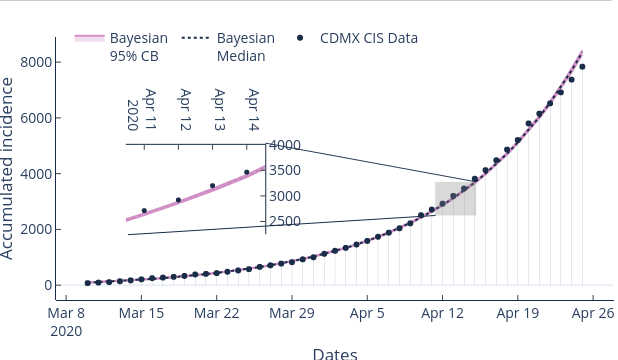
\includegraphics[width=0.8\textwidth, keepaspectratio]{%
			assets/MCMC_CDMXDataFitting.png%
		}
		\caption{%
			MCMC Fit of diary new cases of Mexico city
			during exponential growth. See
			\url{https://plotly.com/~sauld/53/} for an electronic
			version.
		}
		\label{fig:data_CDMX_fitting}
	\end{figure}
\end{frame}


        \subsection{Aims, methodology, and contribution}
            \begin{frame}{Aims, methodology, and contribution}
    \begin{textblock*}{80mm}(5mm,10mm)
        \only<1->{
            \begin{description}
                \item[Aim:]
                    Improve the estimation of the infection rates
                    $\beta_s$, $\beta_a$, and ratio of asymptomatic cases $p$.
                \item[Hypothesis:]
                    Noise could improve the
                    uncertainty quantification.
            \end{description}
        }
    \end{textblock*}
    \begin{textblock*}{55mm}(5mm,30mm)
        \only<2->{
            \begin{graybox}{
    	   Solution idea:
            }
                \begin{itemize}[label= \textbullet]
                    \item Deterministic Inference
                        \begin{itemize}[label= \ding{51}]
                            \item ODE 
                            \item MCMC
                        \end{itemize}
                    \item Stochastic Inference
                        \begin{itemize}[label= \ding{113}]
                            \item SDE extension
                            \item Lamperti
                            \item Grisanov
                            \item Opt. ML 
                        \end{itemize}
                \end{itemize}   
            \end{graybox}
        }
    \end{textblock*}
    \begin{textblock*}{50mm}(70mm,35mm)
        \only<3>{
            \begin{greenbox}{Contribution}
                \begin{itemize}[label = \ding{217}]
    			\item 
                        A stochastic SEIR.
                    \item 
    				Consistent estimators.
    			\item 
    				Simulation.
        \item 
         Real data.
     		\end{itemize}
            \end{greenbox}
        }
    \end{textblock*}
\end{frame}	

\begin{bibunit}[apalike]
    \begin{frame}{Our Contribution \cite{Baltazar2022}}
        \biblio{main}
    \end{frame}
\end{bibunit}
                \subsection{Related Work}
            \begin{bibunit}[plain]
	\begin{frame}{Related Work}
		
		\begin{textblock*}{120mm}(5mm, 10mm)
				Works that report estimation for SDE models for similar structures (SIS,or SIR) and  with only numeric experiments of synthetic nature. Complex stochastic models similar to the one considered here that are only studied on a theoretical basis and/or with numerical simulations but without estimations methods.	
		\end{textblock*}
	%	
		\begin{textblock*}{40mm}(0mm,30mm)
			\small{
			\begin{itemize}[label = $\dagger$]
				\item 
					\cite{Ndanguza2016} focus on the 
					calibration parameters 
					by adaptive MCMC and extended Kalman filter methods. 
				\item
					\cite{Hotta2010}
					report other Bayesian techniques, 
				\item \cite{Rios2021}
					apply a maximum likelihood method and
				\item
					\cite{Otunuga2021} 
					reports a parameter estimation with 
					local generalized methods of moments.
			\end{itemize}
			}
		\end{textblock*}
		\begin{textblock*}{90mm}(40mm,30mm)
			\scalebox{0.8}{
				\begin{minipage}{1.20\textwidth}
					\biblio{main}
				\end{minipage}
			}
		\end{textblock*}
	\end{frame}
\end{bibunit}
                \begin{frame}
                   \frametitle{Table of contents}
                   \tableofcontents
                \end{frame}
            \subsection{
                Stochastic Formulation by Perturbation of parameters
            }
                \begin{frame}{Stochastic perturbation}
	\begin{textblock*}{60mm}(10mm, 15mm)
		Perturbing the above deterministic base by Brownian Motion
	\end{textblock*}
	%
	\begin{textblock*}{100mm}(20mm, 30mm)
		\begin{graybox}{
				$\mu dt\rightsquigarrow \mu dt + \sigma dW(t)$ gives
				our SDE SEIR-Covid-19
			}
			\begin{equation*}
				\begin{aligned}
					d {S}(t)  =&
					\big[\mu - \mu S(t) - f_{\beta} S(t)
					+\gamma R(t)  \big] dt 
					+ \color{orange}{
						\sigma \big(1- S(t)\big) dW(t)
					}
					\\
					d {E}(t) =& \big[  f_{\beta} S(t)
					- \kappa  E(t) - \mu E(t) \big] dt  
					- \color{orange}{
						\sigma E(t) dW(t)
					}
					\\
					d {I_a}(t) =& \big[
					p \kappa E(t)
					-   (\alpha_a +\mu) I_a(t)  \big] dt  
					- \color{orange}{
						\sigma I_a(t) dW(t)
					}
					\\
					d {I_s}(t) =& \big[
					(1 - p) \kappa E (t)
					- (\alpha_s +\mu)  I_s(t) \big] dt   
					- \color{orange}{
						\sigma I_s(t) dW(t)
					}
					\\
					d {R}(t) =&
					\big[
					\alpha_a I_a(t) +
					\alpha_s I_s(t) - (\mu + \gamma) R(t)
					\big] dt
					- 
					\color{orange}{
						\sigma R(t) dW(t)
					},
					\\
					& t \in  [0, T] .
				\end{aligned}
			\end{equation*}
		\end{graybox}
	\end{textblock*}
\end{frame}
%------------------------------------------------------------------
%------------------------------------------------------------------
\begin{frame}{Grisanov's likelihood ratio}
	Let $\mathbb{P}_{\beta, p}$ the law of solution to SDE. We use the
	following result
	\footnote{%
		S\"arkk\"a, Simo;
		Solin, Arno, Applied stochastic differential
		equations. Institute of Mathematical Statistics Textbooks,
		10. Cambridge University Press, Cambridge, 2019. ix+316 pp.
		ISBN: 978-1-316-64946-6
	}.%
	\begin{theorem}%
		[%
		{%
			Likelihood ratio of Itô processes
			S\"arkk\"a and Solin (2019, Thm. 7.4)%
		}%
		]%
		Consider the It\^o processes
		\begin{equation*}
			\begin{aligned}
				dx =& f(x, t) + dB_t , \qquad x(0) = x_0,
				\\
				dy =& g(y, t) + dB_t, \qquad y(0) = x_0.
			\end{aligned}
		\end{equation*}
		%        where $x(t), y(t) \in \mathbb{R}^D$ and the Brownian motion
		%        $B_t \in \mathbb{R}^D$ has no singular diffusion matrix $\mathbf{Q}$.
		Then the ratio of probability laws of $\mathcal{X}_t$ and
		$\mathcal{Y}_t$ is given as
		\begin{equation*}
			\begin{aligned}
				\frac{p(\mathcal{X}_t)}{p(\mathcal{Y}_t)} =& Z(t),
				\\
				Z(t) =
				\exp \Big(
				-\frac{1}{2}
				&
				\int_0^t
				[f(y, \tau) - g(y, \tau)]^{\top}
				\mathbb{Q}^{-1}
				[f(y, \tau) - g(y, \tau)] d \tau
				\\
				+
				&\int_0^t
				[f(y, \tau) - g(y, \tau)]^{\top}
				\mathbb{Q}^{-1}
				d B_{\tau}
				\Big)
			\end{aligned}
		\end{equation*}
		in the sense that for an arbitrary functional $h(\cdot)$ of the path
		from $0$ to $t$,
		$$
		\EX{h(\mathcal{X}_t)}{} = \EX{Z(t) h (\mathcal{Y}_t)}{}
		$$
	\end{theorem}
\end{frame}
%-------------------------------------------------------------------------------
%-------------------------------------------------------------------------------%
\begin{frame}{The Lamperti transform}
	Suppose we have the SDE
	$$
	dX_t = a(t, X_t) dt + b(X_t) dW_t,
	$$
	where the diffusion coefficient depends only on the state variable.
	Such SDE can transform into one with unitary diffusion by applying the
	\emph{Lamperti} transform
	$$
	Y_t:= F(X_t) = \int_{z} ^ {X_t} \frac{1}{b(u)}du.
	$$
	Here $z$ is an arbitrary value and $Y_t$ solves
	$$
	d Y_{t} = 
	\left(
	\frac{a(t, X_t)}{b(X_t)}
	- \frac{1}{2} b_x (X_t)
	\right) dt
	+ dW_t
	$$
	The results follows form the It\^{o} formula.
\end{frame}
%-------------------------------------------------------------------
\begin{frame}
	\begin{textblock*}{80mm}(0mm, 0mm)
		\begin{graybox}{Using It\^o and Lamperti transformations}
			\scalebox{.7}{%
				\parbox{\linewidth}{%
					\begin{equation*}
						\begin{aligned}
							d {S}(t)  =&
							\big[
							\mu - \mu S(t) - f_{\beta} S(t)
							+ \gamma R(t)
							\big] dt +                                                                
							\sigma \big(1- S(t)\big) dW(t)
							\\
							d {E}(t) =&
							\big[
							f_{\beta} S(t)
							- \kappa  E(t) - \mu E(t)
							\big] dt  - \sigma E(t) dW(t)
							\\
							d {I_a}(t) =&
							\big[
							p \kappa E(t)
							-(\alpha_a +\mu) I_a(t)
							\big] dt  - \sigma I_a(t) dW(t)
							\\
							d {I_s}(t) =&
							\big[
							(1 - p) \kappa E (t)
							- (\alpha_s +\mu)  I_s(t)
							\big] dt
							- \sigma I_s(t) dW(t)
							\\
							d {R}(t) =&
							\big[
							\alpha_a I_a(t) +
							\alpha_s I_s(t) - (\mu + \gamma) R(t)
							\big] dt
							- \sigma R(t) dW(t),
							\\
							& t \in  [0, T] .
						\end{aligned}%
					\end{equation*}
				}
			}
			\tcblower
			$
			-\frac{1}{\sigma}
			d \mathbf{X}_{\beta,p}(t) =
			F\big(\mathbf{X}_{\beta,p}(t)\big) dt + d\mathbf{W}(t),
			$
		\end{graybox}
	\end{textblock*}
	%
	\begin{textblock*}{120mm}(10mm, 50mm)
		\scalebox{.7}{%
			\parbox{\linewidth}{%
				%
				\begin{equation*}
					\mathbf{X}_{\beta,p}(t) :=
					\begin{pmatrix}
						\log \big(1-S(t)\big)
						\\
						\log \big(E(t)\big)
						\\
						\log \big(I_a(t)\big)
						\\
						\log \big(I_s(t)\big)
						\\
						\log\big (R(t)\big)
					\end{pmatrix},
					\quad
					F\big(\mathbf{X}_{\beta,p}(t)\big):=
					\begin{pmatrix}
						\dfrac{\mu}{\sigma } -
						\dfrac{f_\beta S(t) }{\sigma \big(1-S(t)\big)}
						+
						\dfrac{\gamma R(t)}{\sigma \big(1-S(t)\big)}
						+ \tfrac{1}{2} \sigma
						\\
						- \dfrac{f_\beta  S(t)  }{\sigma E(t)}
						+ \dfrac{ \kappa   }{\sigma }
						+ \dfrac{\mu }{\sigma }
						+ \dfrac{1}{2} \sigma
						\\
						- \dfrac{\kappa p E(t)}{\sigma I_a(t)}
						+ \dfrac{(\alpha_a + \mu )}{\sigma }
						+ \dfrac{1}{2} \sigma
						\\
						- \dfrac{\kappa (1-p) E(t)}{\sigma I_s(t)}
						+ \dfrac{(\alpha_s + \mu )}{\sigma }
						+ \dfrac{1}{2} \sigma
						\\
						- \dfrac{\alpha_a I_a(t) +
							\alpha_s I_s(t)}{\sigma
							R(t)}
						+ \dfrac{\mu + \gamma}{\sigma }
						+ \dfrac{1}{2} \sigma
					\end{pmatrix},
					\quad
					d\mathbf{W}(t):=
					\begin{pmatrix}
						dW(t)
						\\
						dW(t)
						\\
						dW(t)
						\\
						dW(t)
						\\
						dW(t)
					\end{pmatrix} .
				\end{equation*}
			}
		}
	\end{textblock*}
\end{frame}
            \section{Statistical Inference}
                \begin{frame}{Statistical Inference: Methodology}
    \begin{itemize}[label=(\ding{43})]
        \item 
            Assume that the true value of the parameters
            $\beta_{s,0}$, $\beta_{a,0}$, $p_0$, and $\sigma_0$ are unknown.
        \item 
            Use the quadratic variation of the SDE solution to estimate $\sigma$. 
        \item 
            Rewrite the SDEs by applying Lamperti's 
            transformation to each component.
        \item  
            Apply the Girsanov formula 
            for the new system, and we obtained the likelihood function and the MLEs for 
            $\beta_{s,0},\beta_{a,0}, p_0$.
    \end{itemize}
\end{frame}

 \begin{frame}{Estimator of the parameter of diffusion $\sigma$}
    \begin{equation*}\label{est_sigma}
        \hat{\sigma}^2:=\sum_{i=1}^5\frac{\hat{\sigma}^2_i}{5},
    \end{equation*}
    where
        \begin{equation*}
            \begin{aligned}
                &\hat{\sigma}^2_1
                  = \frac{<S,S>_T}{\int_0^T(1-S(t))^2dt},
                \qquad
                \hat{\sigma}^2_2
                    = \frac{<E,E>_T}{\int_0^TE(t)^2dt},
                \qquad
                \hat{\sigma}^2_3
                    = \frac{<I_a,I_a>_T}{\int_0^TI_a(t)^2dt},
                \\
                    & \hat{\sigma}^2_4
                    = \frac{<I_s,I_s>_T}{\int_0^TI_s(t)^2dt},
                    \qquad
                    \hat{\sigma}^2_5
                    = \frac{<R,R>_T}{\int_0^TR(t)^2dt}.
            \end{aligned}  
        \end{equation*}
\end{frame}
%--------------------------------------------------------------------
\begin{frame}{MLEs for infection rates }
        \begin{equation*}
            \begin{pmatrix}
                 \hat{\beta_s}  
                 \\
                 \hat{\beta_a} 
            \end{pmatrix}
        =
            - \sigma 
        \begin{pmatrix}
            J_s(T) & J_{sa}(T)\\
            J_{sa}(T & J_a(T)
        \end{pmatrix}^{-1} \, 
        \begin{pmatrix}
            \int_0^T 
                \Big[ 
                    \dfrac{S(t) I_s(t)}{ (1-S(t))} 
                    + \dfrac{S(t) I_s(t)}{ E(t)} 
                \Big] 
             dW(t) 
         \\
         \int_0^T 
             \Big[
                 \dfrac{S(t) I_a(t)}{ (1-S(t))}
                 + \dfrac{S(t) I_a(t)}{ E(t)} 
             \Big]  dW(t)
        \end{pmatrix}.
    \end{equation*}
    whith
    \begin{align*}
        J_\star(T)
            &:= 
                \int_0^T 
                    \left(
                        \Big[
                            \dfrac{S(t) I_\star(t)}{ (1-S(t))} 
                        \Big]^2  
                        +
                        \Big[ 
                            \dfrac{S(t) I_\star(t)}{ E(t)}
                        \Big]^2 
                    \right) dt,
        \\
        J_{sa}(T)
            &:=  
                \int_0^T 
                    I_a(t) I_s(t) 
                    \left(
                        \Big[
                            \dfrac{S(t)}{(1-S(t))}
                        \Big] ^ 2  
                        +
                        \Big[
                            \dfrac{S(t)}{E(t)} 
                        \Big] ^ 2 
                    \right) dt.
    \end{align*}
\end{frame}
%
\begin{frame}{MLE for proportion of asymptomatic }
    \begin{align*}
         \label{MLE_p}
         \hat{p}_{ML}&=
             \frac{\sigma }{J_2(T)} 
                 \int_0^T 
                     \Big[
                         - \dfrac{\kappa E(t)}{ I_a(t)} 
                         + \dfrac{\kappa E(t)}{ I_s(t)} 
                     \Big] dW(t),
    \end{align*}
 with 
$$
    J_2(T):=
        \int_0^T
            \Big[
                \dfrac{\kappa ^ 2 E ^ 2(t)}{I_s^2(t)} 
                + \dfrac{\kappa ^ 2 E ^ 2(t)}{ I_a^2(t)}
            \Big] dt.
$$
\end{frame}
%-------------------------------------------------------------------------


\begin{frame}{Consistency of our estimators}
\textbf{Hypotheses}
    There exists $T_0>0$ such that for all $t\in [0,T_0]$
     \begin{itemize}[label=(\ding{109})]
         \item
             $\mathcal{R}_0 ^ D > 1$ where 
             $$
                 \mathcal{R}_0^{D}:= 
                 \dfrac{p \kappa \beta_s }{(\mu + \kappa) (\mu + \alpha_s)}
                 +
                 \dfrac{(1 - p) \kappa \beta_a}{
                     (\mu + \kappa)(\mu + \alpha_a)}.
             $$
         \item
            The initial condition $X_0 ^ +$ and parameter configuration 
            $\varphi$ are such that ${\Omega^* \neq  \emptyset}$ where
            \begin{equation*}
                \begin{aligned}
                    \Omega^{*} :=
                    \left \{
                        (S, E, I_a, I_s, R) \times [t_0 , T]:
                    \right.
                    &
                    S(T) \leq S(t) < S(t_0),
                    \\
                     &
                    \left.
                     E(t) > E(t_0), \ 
                     I_a(t) > I_a(t_0), \ 
                     I_s(t) > I_s(t_0)
                     \right \}.
                \end{aligned}
            \end{equation*}
        \end{itemize} 
    \begin{theorem}\label{Consitency-th}
       
        The estimators 
        $(\hat{\beta}_{s,ML},\hat{\beta}_{a,ML},\hat{p}_{ML})$ 
        are  strongly consistent; that is,
        \begin{equation}
            \label{consistency}
            \lim_{T \rightarrow T_0} 
            \begin{pmatrix}
                \hat \beta_{s,ML} 
                \\
                \hat \beta_{a,ML} 
                \\
                \hat p_{ML}
            \end{pmatrix}
            = 
            \begin{pmatrix}
                \beta_{s,0} 
            \\
                \beta_{a,0} 
            \\
                p_0
            \end{pmatrix}, 
            \qquad \mbox{with probability one.}
        \end{equation}
    \end{theorem}
    See \cite{Baltazar2022}
\end{frame}
    %
            \section{Simulation study}
                \begin{frame}{Parameters of the simulation}
\begin{itemize}
\item Using the Milstein scheme, we divide the interval $[0,T]$ into $n$ sub-intervals of length 
$\Delta=\frac{T}{n}$ and we obtain observations of each process at the times 
$0=t_0<t_1<\ldots<t_n=T$ where $t_i-t_{i-1}=\Delta, i=1,\ldots,n$.
\item We simulate a 1000 datasets in the time interval $[0,1]$. 
    We use 
    $   \beta_a=0.251521
    $,
    $
        \beta_s=0.456391
    $,
    $
        p=0.1213
    $,
    $
        \sigma=1/5000
    $, values of Table \ref{table:parametermodel} and $\Delta=1/850$.
      

\end{itemize}
\end{frame}

\begin{frame}{Estimator of simulation study}
    \begin{table}[tbh]
        \centering
        \begin{tabular}{rlcc}\hline
Parameter & Real Value & Estimator & SD \\ \hline 
             $\beta_s$ & 0.456391 & 0.453155 & 2.900549E-005\\
            $\beta_a$  & 0.251521 & 0.265229 & 6.081389E-002  \\
    $p$ & 0.1213&0.120354 & 2.554605E-006\\          
    $\sigma$ & 1/5000 & 1.361178E-004 & 5.325816E-009\\
            \hline
        \end{tabular}
        \caption{Average and  Standard Deviation (SD) of estimator of $\sigma$ and MLEs for $\beta_a,\beta_s$, and $p$.}
        \label{table:MLE}
    \end{table}

    \end{frame}

    %\section{Parameter estimation of SEIR-Covid-19 model based on a SDE}
    \section{Application to real data}
             \begin{frame}{Data description}
     \begin{itemize}[label=*]
        \item 
            we use the dataset of new symptomatic and 
            confirmed COVID-19 reported cases daily in Mexico City, considering 
            that its population is $N=26446435$.
        \item 
            The dataset contains 
            47 records in the period March 10 to April 25, 2020.
        \item  
            We use 
            these records $I^o_s$ to construct the observations, the process 
            $I_s:=I^o_s/N$.  
        \item  
            Combining $I_s$ and the Milstein scheme, we generate the
            others four processes of the system  with the parameters of Table
            \ref{table:parametermodel}, 
            $\sigma=1/100$ and $\Delta=1/1000$.
    \end{itemize}
\end{frame}
%------------------------------------------------------------------------------
\begin{frame}{Data construction }
    \begin{algorithm}[H]
        \caption{Construction of dataset.} \label{Alg-ds}  
        \begin{algorithmic}[1]
            \State Using initial conditions and make $n=0$.
            \State Generate 
                $\Delta W\sim N(0,\Delta)$.
            \State 
                $
                    S(t_{n+1}) = 
                        S(t_n) - (\mu+\beta_aI_a(t_{n}) 
                        + \beta_s I_s^{mx}(t_n))\Delta S(t_{n}) 
                        + (\mu+\gamma R(t_n)) * \Delta 
                        - \sigma(1-S(t_n))\Delta W
                $
            \State 
                $
                    E(t_{n+1}) = E(t_{n}) - (\kappa+\mu) * \Delta E(t_{n}) 
                    + \Delta * (\beta_sI_s ^ {mx}(t_n) 
                    + \beta_aI_a(t_{n})S(t_n)
                    - \sigma(E(t_n))\Delta W
                $
            \State 
                $
                    I_a(t_{n+1}) = I_a(t_{n}) 
                        - p\kappa E(t_{n}) \Delta I_a(t_{n})
                        - (\alpha_a+\mu)I_a(t_{n})\Delta
                        - \sigma I_a(t_{n})\Delta
                $
            \State 
                $
                    R(t_{n+1}) = 1 - S(t_{n+1}
                        - E(t_{n+1}) - I_a(t_{n+1})
                        - I^{mx}_s(t_{n+1})
                $.
            \State If $n<47$ make $n=n+1$ and go to 2. In other case stop.
        \end{algorithmic}
    \end{algorithm}
\end{frame}
%-------------------------------------------------------------------------------
%  \begin{frame}{Initial conditions}
% \begin{table}[tbh]
%         \centering
%         \begin{tabular}{
%             rl  
%         }
%             \hline
%             Process & Value
%             \\
%           \hline
            
%             $E(0)$ & 198.504525/N
                 
%             \\
%             $I_a(0)$ & 
%                 99.174034/N
%             \\
%             $I_s(0)$ & 74/N
                
%             \\
               
%             $R(0)$ & 
%                 0 
%             \\
%             $S(0)$ &  $1-(E(0)+I_a(0)+I_s(0)+R(0))$ 
%             \\      
        
%            \hline
%         \end{tabular}
%         \caption{Initial Conditions.}
%         \label{table:initial}
%     \end{table}
%     \end{frame}

\subsection{Estimation of parameters}
\begin{frame}{Estimators for real data}
    We assume the following parameters as given:
    $\gamma =1 /365$,
    $\kappa = 0.196078$,
    $\alpha_a = 0.167504$ 
    $\alpha_s = 0.092507$. 
    We generate 1000 datasets using the data of Mexico City. 
    \begin{table}[tbh]
        \centering
        \begin{tabular}{%w
                %>{\centering}
                %p{1in}
                %p{3in}
                %p{0.57\textwidth}
            rccc
        }
            \hline
            Parameter  & Estimator & CIL & CIU
            \\
              \hline
            
            $\beta_s$ 
            
            &  0.059159 & 0.002546&
            0.115772
            \\
            $\beta_a$ 
        
            & 0.509925 & 0.378248 &
            0.641603
            \\
        
            $p$ 
            
            &0.582808 &0.582326&0.583289
            \\          
            $\sigma$ & 1.31701E-002
            & 8.32156E-003&
            1.94434E-002\\
                  \hline
        \end{tabular}
        \caption{
            Average and  95\% confidence interval of the estimator of 
            $\sigma$ and MLEs for $\beta_a,\beta_s$, and $p$.
        }
        \label{table:MLEREAL}
    \end{table}
\end{frame}
%-------------------------------------------------------------------------------------------
\begin{frame}
    \begin{figure}[htb]
        \centering
        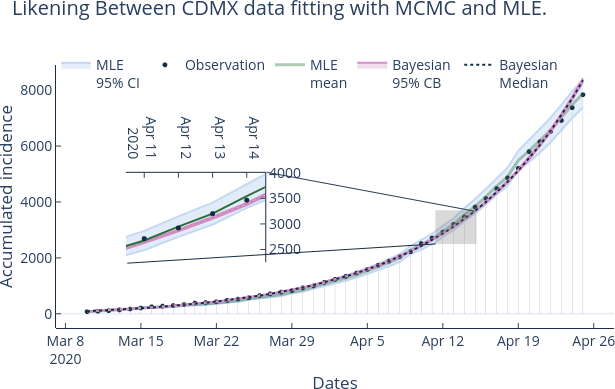
\includegraphics[width=1.0\textwidth, keepaspectratio]{assets/Likening.png}
     
        \label{fig:real_data_fitting}
    \end{figure}    
\end{frame}
%--------------------------------------------------------------------------------------------

\subsection{Validation of the model}
\begin{frame}{Validation of the model}
    \begin{figure}[htb]
        \centering
        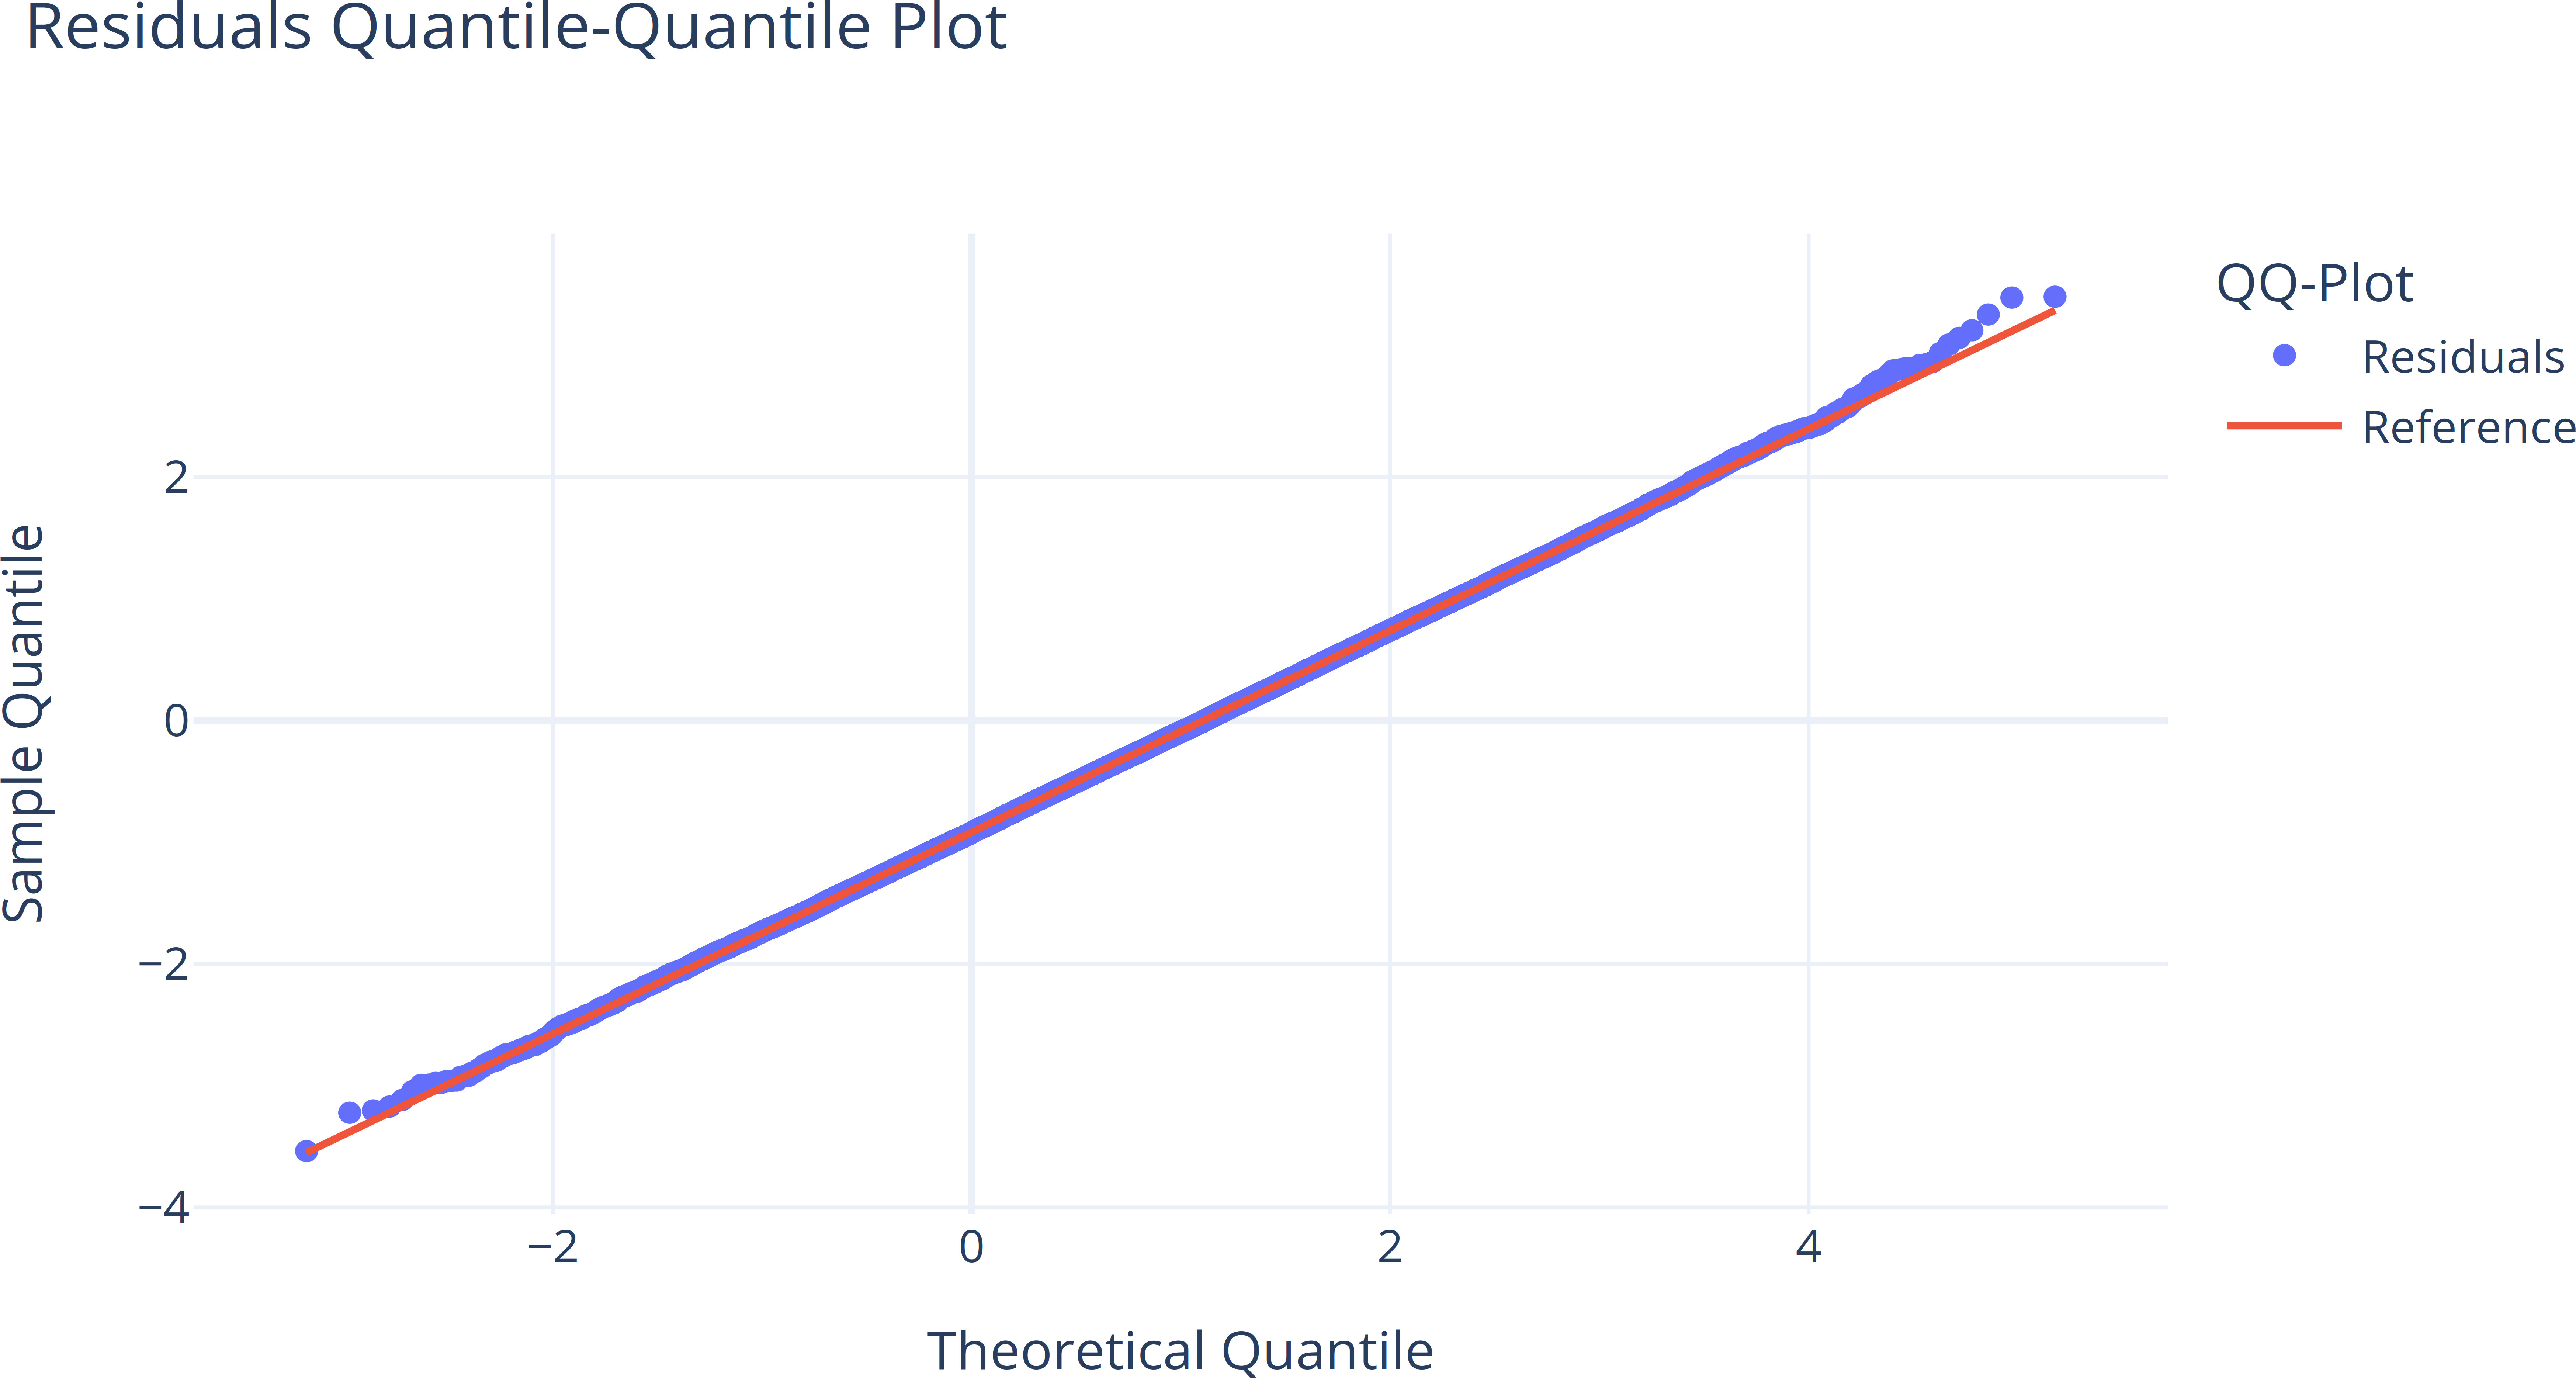
\includegraphics[scale=0.6]{assets/qq_plot.png}
        \caption{Quantile-Quantile plot of the numerical residuals.}
         \label{fig:fig_qq}
     \end{figure}
\end{frame}
    %\section{Final comments}
    %
    %\begin{frame}[allowframebreaks]
    %   \frametitle{Final Remarks}            
    %    \bibliographystyle{acm}
    %    \bibliography{main.bib}
    %\end{frame}
\end{document}
